\chapter{System Implementation}
\label{Ch-5:Sec:System}

In this chapter, we'll combine the work of \nameref{Ch-2:Sec:Standardize} and \nameref{Ch-3:Sec:Extraction}. A data visualization task is also include in this chapter. 

\section{Frame of System}

\begin{figure}
	\centering
	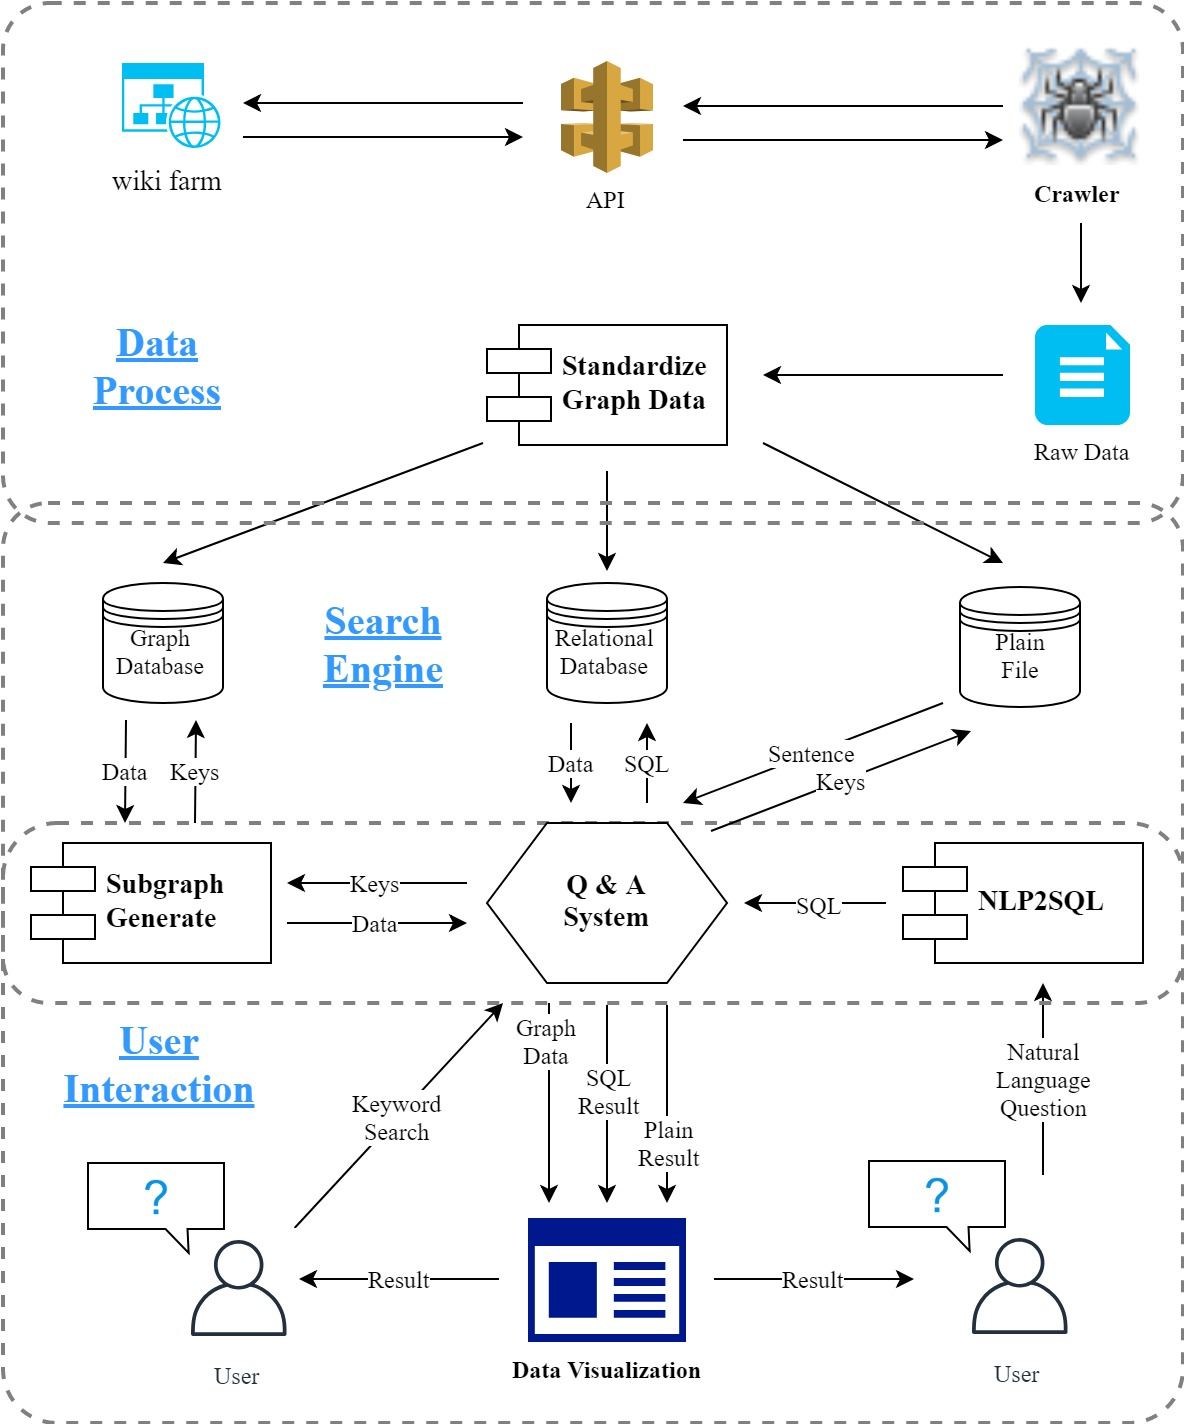
\includegraphics[width=0.8\linewidth]{fig/Section5.jpg}
	\caption{The Structure of System Implementation}
	\label{fig:section5-pic1}
\end{figure}

The flow chart \nameref{fig:section5-pic1} illustrates the frame of whole project. The Q \& A system is separated in three parts:
\begin{enumerate}
	\item Data Process, including data crawling, data cleaning, data storing and data standardizing, referring to the work in\nameref{Ch-2:Sec:Standardize}.
	\item Search Engine, including subgraph generating, natural language processing and APIs with 3 databases, referring to the work in\nameref{Ch-3:Sec:Extraction}.
	\item Data Visualization, including user Interface, Q \& A system module, APIs with search engine and enhancing user search results.
\end{enumerate}

\section{Summary of Technique}

We use \href{https://plot.ly/}{Plotly}\footnote{https://plot.ly/} and \href{https://plot.ly/products/dash/}{Dash}\footnote{https://plot.ly/products/dash/} for the data visualization task. They're modern analytics apps which can build beautiful web-based interfaces in Python. \\
At first, the project is built on Kivy with igraph.plot. However, the interaction between these two packages can't realize what we desire. Different purposes with different builders influence their compatibility. It's hard to build a dynamic graph which can interact with users. Thus, we decide to search for other tools to solve the data visualization tasks.\\
Scatter3d component is used for graph data plotting and user interaction. HTML components are used for listing text answers. Dropdown and input components are also used for user interaction.

\section{Conclusion}
(unfinished)